\chapter{Structural typology description}
When it comes to building the terminal, it is important to specify which kind of materials are going to be used, and thus, the efforts that will hold the structure. In a general frame, it can be distinguished between two types of mechanisms of effort transmission to the foundation; firstly, the vertical efforts due to the gravitational load and, secondly, the lateral efforts due to the wind or possible earthquakes.

In the first case, the load-bearing elements work in compression and the ceilings work in bending-shear in the manner of a beam subjected to perpendicular loads in its plane.

In the second case, the same elements act differently. The ceilings receive and accumulate horizontal forces, working as a membrane and distributing forces between the different vertical elements, while the vertical elements work to bending-shear.

	\section{Foundation}
Indonesia is a country with a very varied terrain due to the numerous geological faults combined with significant erosion. Volcanoes are the spine of Java. This irregular chain of volcanoes, which spread over the entire length of the island, forms the most active part of the 'Ring of Fire' volcano chain. The volcanism typical of Java's Island corresponds to the alkaline series, in which basalts, tephrites and phonolites predominate. Moreover, the zone is full of subterranean activity, earthquakes are fairly common. Most of them are not very powerful but it is very important to take into account this phenomena in terms of building the foundations.

The Island of Java is a region located in a area close to the coast, which implies the abundance of swampy land. Therefore, a deep foundation will be carried out in front of a medium or superficial one, since the superficial terrain will not be able to absorb the efforts that will transmit through a direct foundation.

Once selected the deep foundation method, it is proceed to define the geometry of the piles with which this foundation will be done. The piles to be used will be cylindrical and the relationship established between its height (H) and radius (R) in order to assure the consistency of the foundation is the following one:

\begin{equation}
\frac{Height}{Radius}>15
\end{equation}

Usually, the height values of the piles will not exceed the 40 meters. From a conservative point of view, it has been selected a height of 35 meters and a base of radius 2.25 meters, which corresponds to a H/R factor of 15.55.

The last step to finish the foundation is to decide whether they are constructed with in situ piles or pre-fabricated ones. In the first case, piles in situ are better than the others in terms of acoustic pollution produced during its installation, but when it comes to low quality construction terrains it can not be the best solution. On the other hand, and therefore the remaining option, is the use of prefabricated piles, which are placed directly. The inconvenience is that this system requires the transport of the previously built piles to the site in which the foundation will be done. Moreover, it is important to take into account the very intense noise and vibrations this process will produce. Although the mechanism of intrusion of the piles by pressure is not suitable for all types of terrains, it is the appropriate method to build the foundations due to the characteristics of the region.

\begin{figure}[H]
	\centering
	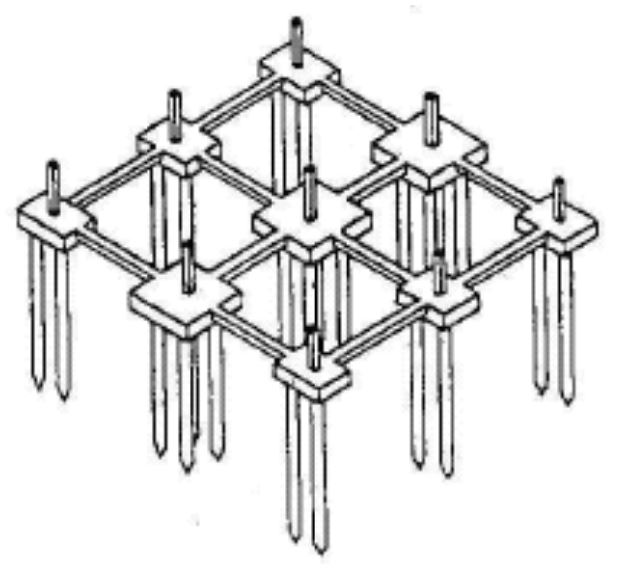
\includegraphics[clip, trim=0cm 0cm 0cm 0cm, width=0.4\textwidth]{./images/TipologiaEstructural/foundationprefabricated}
	\caption{Schema of deep foundation with prefabricated piles.}
	\label{foundation}
\end{figure}

	\section{Vertical elements}
The pillars are the resistant elements responsible for supporting mainly compression loads in a vertical direction and also can absorb small lateral bending loads. The main function of them is to distribute the loads of the ceiling and the slabs to the foundation. It is important to remark that there is an alternative of vertical resistant elements, which are the loading walls but in case of Bekasi-East Jakarta Airport this solution will not be carried out.

The basic types of pillars found in construction are in situ reinforced concrete, prefabricated concrete, metal structure and mixed structure of steel and concrete. In the case of the new airport's terminal building, it is decided to make the pillars with mixed structure of steel and concrete. In this way, the pillars will have smaller sections than the those made of in situ reinforced concrete and will have more fire resistance than the metallic ones. Moreover, this type of pillars work very well in front of earthquakes, since the metallic armor is able to support the efforts in order to maintain the building up.

Starting from the foundation, the pillars of the ground floor will have a considerable section, since they will have to support greater loads and  weight of the structure.

On the ground floor, in order to support the slab, pillars made of reinforced concrete will be used. The diameter of them will be 1 meter.

As far as the upper floor is concerned, some of the pillars from the ground floor will be extended to this level. At the level mentioned, it will not be necessary to place the same number of pillars as in the ground floor, since the structure in this case has to support less efforts and weight.

The distribution of the pillars can be seen in the drawings of the airport attached to the documents.

	\section{Slab}
The slab is the horizontal structural element that directly receives the loads and transmits them to the remaining elements of the structure. Before deciding what type of slab will be used in the terminal building it is necessary to know the
functions of it:

\begin{itemize}
		\item Support itself and the loads received
		\item Support the construction process
		\item Solidarize all the elements of the plants
		\item Distribute the horizontal loads between all the elements
		\item Present compatibility of deformations with their functions
		\item Isolate the plants thermally and acoustically
		\item Resist to fire
\end{itemize}

It is also important to differentiate between types of slabs. It can be found unidirectional slabs, usually prefabricated or made of beams and vaults, and bidirectional, which can be waffle slabs or solid slabs.

Having a look to these different types of slabs, it is decided that the best option to the new airport terminal building will be a bidirectional waffle slab which will provide a bi-dimensional loads distribution. They are flat slabs without beams, composed of nerves in two directions, which can be built with recoverable moulds or with permanent lightening. The waffle slab must be filled with reinforced concrete and later framed. This process implies the need of approximately 28 days to be ready. The waffle frame allows to have higher lights than other ones and, in addition, there is no problem concerning its transportation, since it is built using in situ reinforced concrete.

\begin{figure}[H]
	\centering
	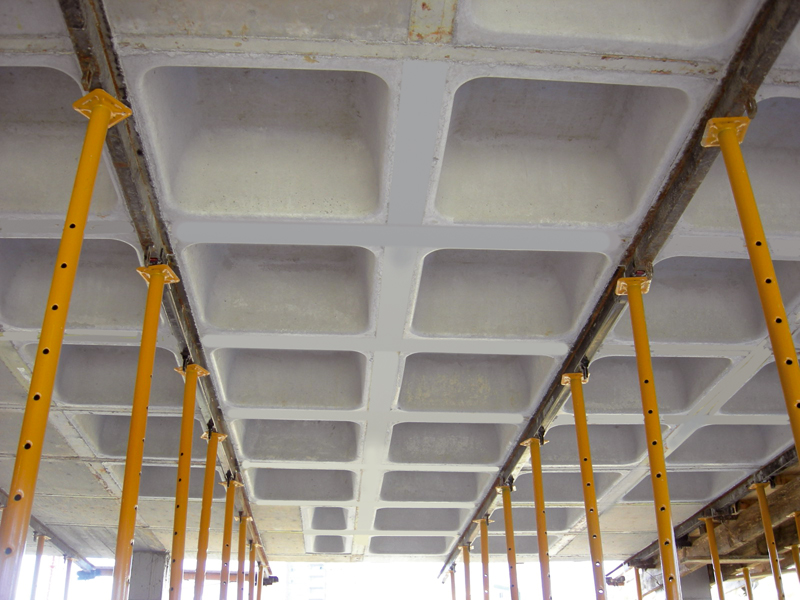
\includegraphics[clip, trim=0cm 0cm 0cm 0cm, width=0.5\textwidth]{./images/TipologiaEstructural/waffleslab}
	\caption{Example of bidirectional waffle slab.}
	\label{slab}
\end{figure}



	
